\section{Serial Data Transfer}

\begin{concept}{Overview}
    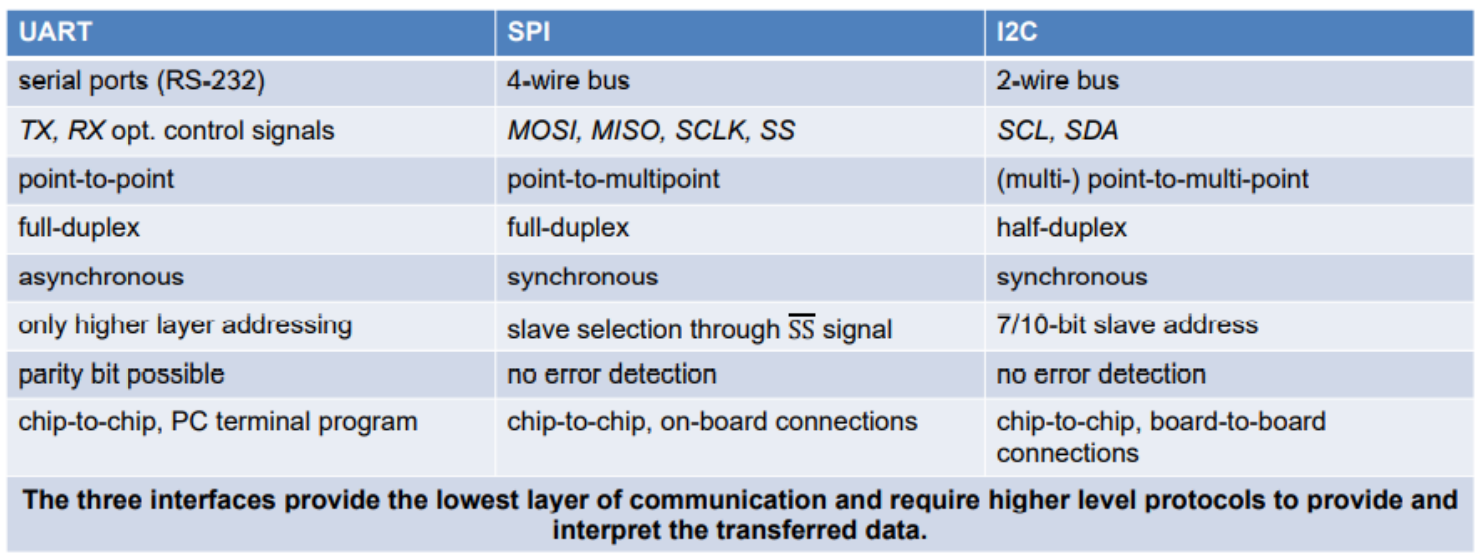
\includegraphics[width=\linewidth]{SDT_overview.png}
    \vspace{2mm}\\
    \textbf{SPI - Serial Peripheral Interface}
    \begin{itemize}
        \item Master/slave
        \item Synchronous full-duplex transmissions (MOSI, MISO)
        \item Selection of device through Slave Select (SS)
        \item no acknowledge, no error detection
        \item Clock signal (SCK) for synchronization: four mode $\rightarrow$ CPOL (clock polarity), CPHA (clock phase)
    \end{itemize}
    \vspace{2mm}

    \textbf{UART - Universal Asynchronous Receiver Transmitter} (Serial Interface)
    \begin{itemize}
        \item Transmitter and receiver use diverging clocks
        \item synchronization using start and stop bits $\rightarrow$ overhead
        \item longer connections require line drivers $\rightarrow$ RS-232/RS-485
    \end{itemize}
    \vspace{2mm}

    \textbf{I2C - Inter-Integrated Circuit}
    \begin{itemize}
        \item Synchronous half-duplex transmission (SCL, SDA)
        \item 7-bit slave addresses
        \item Acknowledge, error detection
        \item Clock signal (SCL) for synchronization
    \end{itemize}
\end{concept}

\begin{definition}{Single Master - Multiple Slaves}
    \begin{itemize}
        \item Master generates a common clock signal for all Slaves
        \item MOSI: From Master Output to all Slave Inputs
        \item MISO: From Master Input to all Slave Outputs $\rightarrow$ all slave outpuzs connected to single master input
        \item Slaves: Selectable by Slave Select (SS) signal
        \begin{itemize}
            \item Individual Select $\overline{SS1}$, $\overline{SS2}$, $\overline{SS3}$
            \item $\overline{SSx}$ = 1 $\rightarrow$ slave output MISOx is tri-state 
        \end{itemize}
    \end{itemize}
    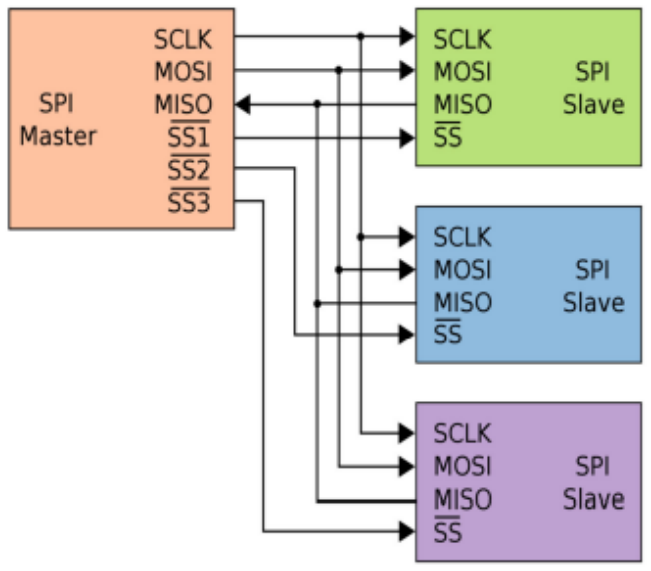
\includegraphics[width=\linewidth]{single_master_mult_slaves.png}
\end{definition}

\begin{formula}{Clock Polarity (CPOL) Clock Phase (CPHA)}
    \begin{itemize}
        \item \textbf{CPOL:} Clock Polarity
        \begin{itemize}
            \item 0: Clock is low in idle state
            \item 1: Clock is high in idle state
        \end{itemize}
        \item \textbf{CPHA:} Clock Phase
        \begin{itemize}
            \item 0: Data is sampled on the first edge of the clock
            \item 1: Data is sampled on the second edge of the clock
        \end{itemize}
    \end{itemize}
    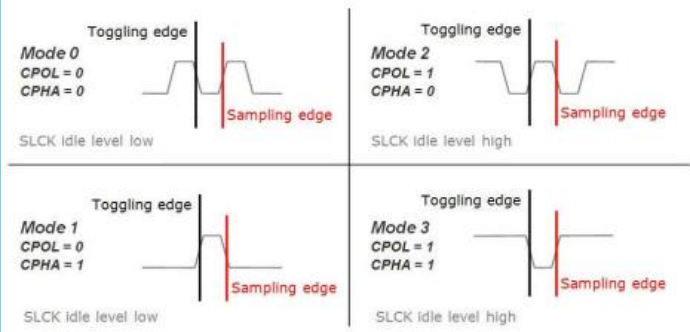
\includegraphics[width=\linewidth]{clockpolarity.png}
    \begin{itemize}
        \item TX provides data on \oq Toggling Edge\cq
        \item RX takes over data with \oq Sampling Edge\cq
    \end{itemize}
\end{formula}

\subsection{Serial Connection - SPI}

\begin{definition}{Properties of SPI}
    \begin{itemize}
        \item No defined addressing scheme
        \begin{itemize}
            \item Use of $\overline{SS}$ instead $\rightarrow$ KISS (Keep It Simple Stupid)
        \end{itemize}
        \item Transmission without receive acknowledge and error detection
        \begin{itemize}
            \item Has to be implemented in higher level protocols
        \end{itemize}
        \item Originally used only for transmission of single bytes
        \begin{itemize}
            \item $\overline{SS}$ deactivated after each byte
            \item Today also used for streams 
        \end{itemize}
        \item Data rate: Highly flexible as clock signal is transmitted
        \item No flow-control available
        \begin{itemize}
            \item Master can delay the next clock edge
            \item Slave can't influence the data rate
        \end{itemize}
        \item Susceptible to noise (spikes on clock signal)
    \end{itemize}
\end{definition}

\begin{example2}{SPI - Serial Peripheral Interface}\\
    Ein Prozessor (SPI Master) sendet das Byte 0x3D = 0011 1101\\
    Die Schnittstelle ist wie folgt konfiguriert:\\
    Mode = 3, CPOL = 1, CPHA = 1, MSB first\\
    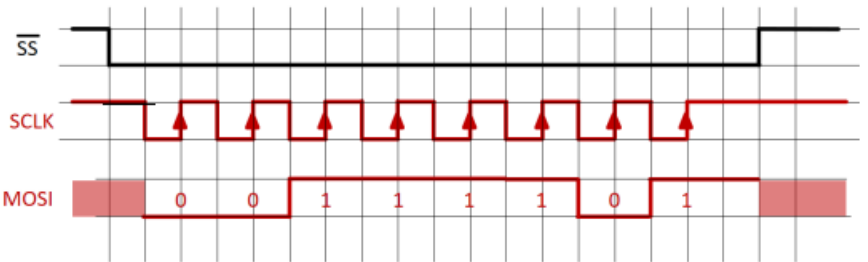
\includegraphics[width=\linewidth]{spi_example.png}
\end{example2}

\begin{concept}{Synchronizing Hardware and Software}
    \begin{itemize}
        \item TXE (TX Buffer Empty) $\rightarrow$ Software can write next TX Byte to SPI\_DR
        \item RXNE (RX Buffer Not Empty) $\rightarrow$ a byte has been received. Software can read it from SPI\_DR
        \item BSY (Busy) $\rightarrow$ Transmission in progress
    \end{itemize}
    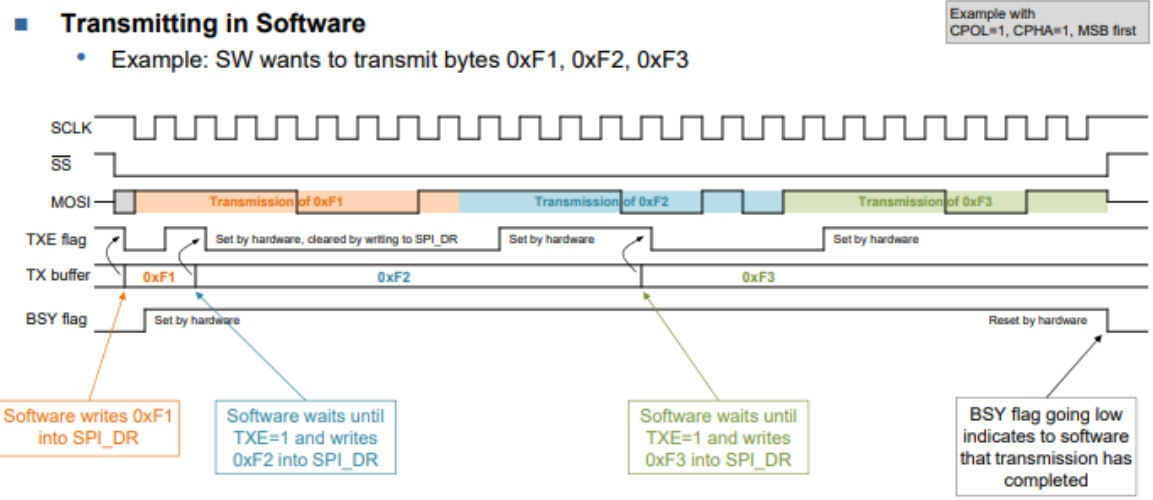
\includegraphics[width=\linewidth]{transmitting_spi.png}\\
    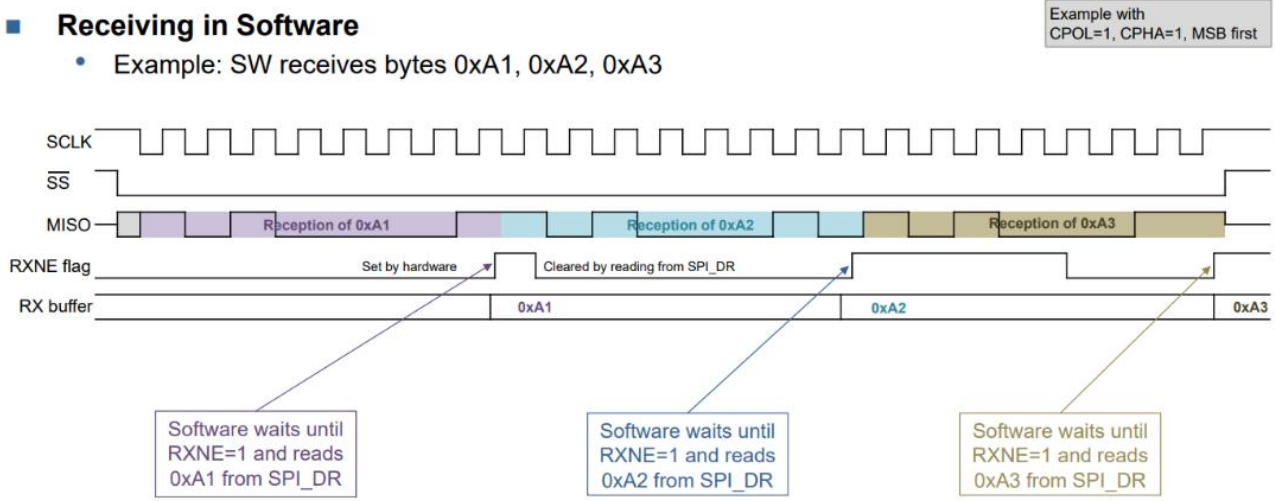
\includegraphics[width=\linewidth]{receiving_spi.png}
\end{concept}

\subsection{UART/I2C}

\begin{definition}{UART - Universal Asynchronous Receiver Transmitter}\\
    Connecting shift registers with diverging clock sources
    \begin{itemize}
        \item same target frequency
        \item different tolerances and divider ratios
        \item requires synchronization at start of each data item receiver
    \end{itemize}
    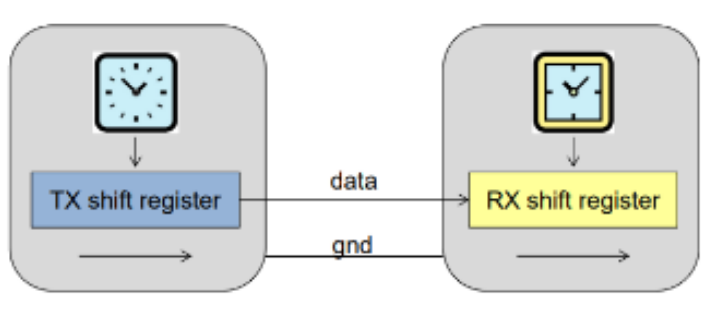
\includegraphics[width=\linewidth]{uart.png}
\end{definition}

\begin{concept}{UART Characteristics}
    \vspace{2mm}\\
    \textbf{synchronization}
    \begin{itemize}
        \item Each data item (5-8 bits) requires synchronization
    \end{itemize}
    \vspace{2mm}

    \textbf{Asynchronous data transfer}
    \begin{itemize}
        \item mismatch of clock frequencies in TX and RX
        \item requires overhead for synchronization $\rightarrow$ additional Bits
        \item requires effort for synchronization $\rightarrow$ additional Hardware
    \end{itemize}
    \vspace{2mm}

    \textbf{Advantages}
    \begin{itemize}
        \item Clock does not have to be transmitted
        \item transmission delays are automatically compensated
        \item no need for a common clock signal
    \end{itemize}
    \vspace{2mm}
    
    \textbf{on-board connections}
    \begin{itemize}
        \item signal levels are 3V or 5V with reference to ground
        \item off-board connections require strong output drivers
    \end{itemize}
\end{concept}

    